\documentclass[sigplan,review,anonymous]{acmart}

% Remove default ACM copyright/conference boilerplate for workshop submission
\settopmatter{printacmref=false}
\renewcommand\footnotetextcopyrightpermission[1]{}
\pagestyle{plain}

% Workshop metadata
\acmConference[AgentSkills'26]{The First Workshop on Agent Skills}{May 26, 2026}{San Jose, CA, USA}
\acmYear{2026}
\copyrightyear{2026}
\acmISBN{}
\acmDOI{}

\usepackage{booktabs}
\usepackage{listings}
\lstset{breaklines=true, basicstyle=\small\ttfamily, language=Python}

\begin{document}

\title{EvolveTool-Bench: Evaluating the Quality of LLM-Generated Tool Libraries as Software Artifacts}

\author{Anonymous Author(s)}
\affiliation{\institution{}}

\begin{abstract}
Modern LLM agents increasingly create their own tools and skills at runtime, from Python functions to API clients, yet existing benchmarks evaluate them almost exclusively by downstream task completion. This is analogous to judging a software engineer only by whether their code runs, ignoring redundancy, regression, and safety. We introduce \textsc{EvolveTool-Bench}, a diagnostic benchmark that evaluates LLM-generated tool and skill libraries as software artifacts. Across three domains requiring actual code execution (proprietary data formats, API orchestration, and numerical computation), we define library-level software quality metrics (reuse, redundancy, composition, regression, and utilization) alongside a per-tool Tool Quality Score measuring correctness, robustness, generality, and code quality. Evaluating four systems spanning the skill-evolution spectrum across 99 tasks and three models (Claude Sonnet 4, Claude Haiku 4.5, and GPT-4o), we show that on Claude models, systems with near-identical task completion (63--68\%) differ by up to 13 percentage points in library health, a gap invisible to task-only evaluation. Across providers, discriminative power varies: GPT-4o converges to identical low performance regardless of evolution strategy, suggesting provider-specific interactions that benchmark designers must account for. Per-dimension analysis reveals that correctness, not code style, is the frontier: hidden tests catch defects that self-generated tests miss. We release the benchmark as an open evaluation framework for any tool-generating or skill-generating system.
\end{abstract}

\maketitle

\section{Introduction}

LLM agents increasingly generate executable software artifacts at runtime (Python functions, API clients, data parsers) and accumulate them in persistent libraries variously called \emph{tools}, \emph{skills}, or \emph{actions}. This capability appears across diverse systems: VOYAGER~\cite{wang2023voyager} synthesizes code skills in Minecraft, CREATOR~\cite{qian2023creator} uses tool creation as a reasoning strategy, LLMs as Tool Makers~\cite{cai2023latm} separates tool-making from tool-using, EvoSkill~\cite{alzubi2026evoskill} evolves structured skill folders via failure analysis, and ARISE~\cite{kaliyev2026arise} provides framework-agnostic middleware for tool synthesis with sandboxed validation. As reusable procedural knowledge is increasingly packaged, shared, and composed across agents, the quality of these generated artifacts becomes a first-order concern.

From a software engineering perspective, each of these systems is an \emph{automated code generator} whose output accumulates into a growing codebase. Yet they are evaluated exclusively on task success, analogous to judging a software engineer solely by whether their code runs, ignoring maintainability, duplication, test coverage, regression, and technical debt. In practice, skill libraries can pass downstream benchmarks while accumulating redundant functions, failing on edge cases, breaking previously working capabilities, and never reusing existing code. Recent work confirms the risk: SkillsBench~\cite{skillsbench2026} found that self-generated skills \emph{hurt} agent performance by 16.2 points in roughly one-third of tasks. \textbf{No existing benchmark measures \emph{why} this happens}: whether the degradation stems from incorrect implementations, redundant code, regression, or failed reuse.

We present \textsc{EvolveTool-Bench}, a diagnostic benchmark that treats LLM-generated tool and skill libraries as software artifacts subject to quality evaluation. The benchmark is system-agnostic: any tool-generating or skill-generating agent can be evaluated against the same tasks and metrics. Our contributions:

\begin{enumerate}
\item \textbf{A metric framework for LLM-generated software artifacts.} We define a per-tool Tool Quality Score (TQS) measuring correctness, robustness, generality, and code quality, plus six library-level metrics: reuse rate, redundancy, quality gate, utilization, composability, and regression stability. Together with safety and refusal cost, these form the EvolveTool Score (ETS), a composite metric that captures both task performance and software quality.

\item \textbf{An evaluation harness with independent validation.} Hidden unit tests and adversarial inputs run in sandboxed subprocesses, providing quality assessment independent of each system's self-validation. Explicit regression tasks measure whether library growth breaks previously working behavior.

\item \textbf{Controlled diagnostic sessions.} Structured sequences of 11 tasks with known dependency relationships (seed, gap, variant, compose, regress, adversarial) enable measurement of reuse recognition, function composition, and library stability as the codebase grows (Figure~\ref{fig:overview}).

\item \textbf{Empirical validation of discriminative power.} We evaluate four systems across three models from two providers and demonstrate that the benchmark reveals quality differences invisible to task completion: per-domain variation, per-dimension TQS distributions, and a ``reuse paradox'' where higher reuse correlates with lower task success.
\end{enumerate}

\section{Related Work}

\paragraph{Quality of LLM-Generated Code.} Tool-Genesis~\cite{xia2026toolgenesis} evaluates one-shot tool creation with surface compliance, schema-F1, and unit test pass rates, all per-artifact metrics with no library-level evaluation. SkillsBench~\cite{skillsbench2026} is the closest work in motivation: it evaluates whether curated skills improve agent task success and finds that self-generated skills \emph{degrade} performance by 16.2 points in $\sim$33\% of tasks, a result that directly motivates our work. However, SkillsBench uses static, pre-curated skill sets and measures only the downstream effect (did performance improve?), not the \emph{cause} (is the skill buggy? redundant? regression-inducing?). Our benchmark complements SkillsBench by providing the diagnostic layer: per-tool quality scores, library-level metrics, and structured sessions that isolate \emph{why} a skill library helps or hurts. Our ``reuse paradox'' (51.9\% incorrect reuse) offers one explanation for SkillsBench's finding: agents reuse skills they correctly identify as relevant but that contain implementation defects. NofunEval~\cite{singhal2024nofuneval} evaluates non-functional aspects of LLM-generated code (efficiency, maintainability) on isolated samples; our work differs by evaluating non-functional properties at the library level, across a growing codebase with reuse and regression. CRAFT~\cite{yuan2023craft} retrieves from specialized toolsets but does not measure the quality of the toolset itself. Berlot-Attwell et al.~\cite{berlotattwell2026} evaluate library learning quality in program synthesis, measuring whether learned abstractions generalize. Their work is similar in spirit to ours, though focused on program synthesis rather than agent skill evolution. None of these works measure redundancy, regression, or reuse across a growing codebase.

\paragraph{Self-Evolving Agent Frameworks.} VOYAGER~\cite{wang2023voyager} demonstrates lifelong skill acquisition in Minecraft, evaluated by exploration metrics. EvoSkill~\cite{alzubi2026evoskill} evolves textual skill folders through failure-driven feedback, evaluated by downstream accuracy. ARISE~\cite{kaliyev2026arise} synthesizes executable Python functions with auto-generated test suites, validates them in isolated sandboxes, and supports iterative refinement. Each generates software artifacts that accumulate into a skill library, but none evaluate the quality of the resulting library, a gap our benchmark fills.

\paragraph{Software Engineering Benchmarks for Agents.} ToolBench~\cite{qin2023toolbench}, AgentBench~\cite{liu2024agentbench}, and ToolComp~\cite{toolcomp2025} evaluate agents using pre-defined tool sets. Vending-Bench~\cite{backlund2025vendingbench} tests long-horizon coherence with fixed tools. None evaluate agents that \emph{generate} their own tools, and none apply software quality metrics to the generated artifacts.

\paragraph{Gap.} No existing benchmark measures redundancy, reuse, regression, composition, or code quality of self-evolved skill libraries as software artifacts. SkillsBench shows that skills can hurt; we provide the diagnostic framework to explain \emph{why}. \textsc{EvolveTool-Bench} fills this gap with a system-agnostic evaluation framework.

\section{Benchmark Design}

We first define key terms used throughout. A \emph{session} is a fixed sequence of 11 tasks executed in order with shared library state. A \emph{task} is a single problem instance presented to the agent, consisting of a natural-language description, expected output format, and verification criteria. The \emph{library} is the persistent collection of Python tools available to the agent during a session, modified when the agent creates or promotes new tools. A \emph{dependency} is a directed relationship where a later task is designed to be solvable using tools created during an earlier task. All tasks require actual Python code execution; no task can be solved by text-only reasoning.

\begin{figure*}[t]
\centering
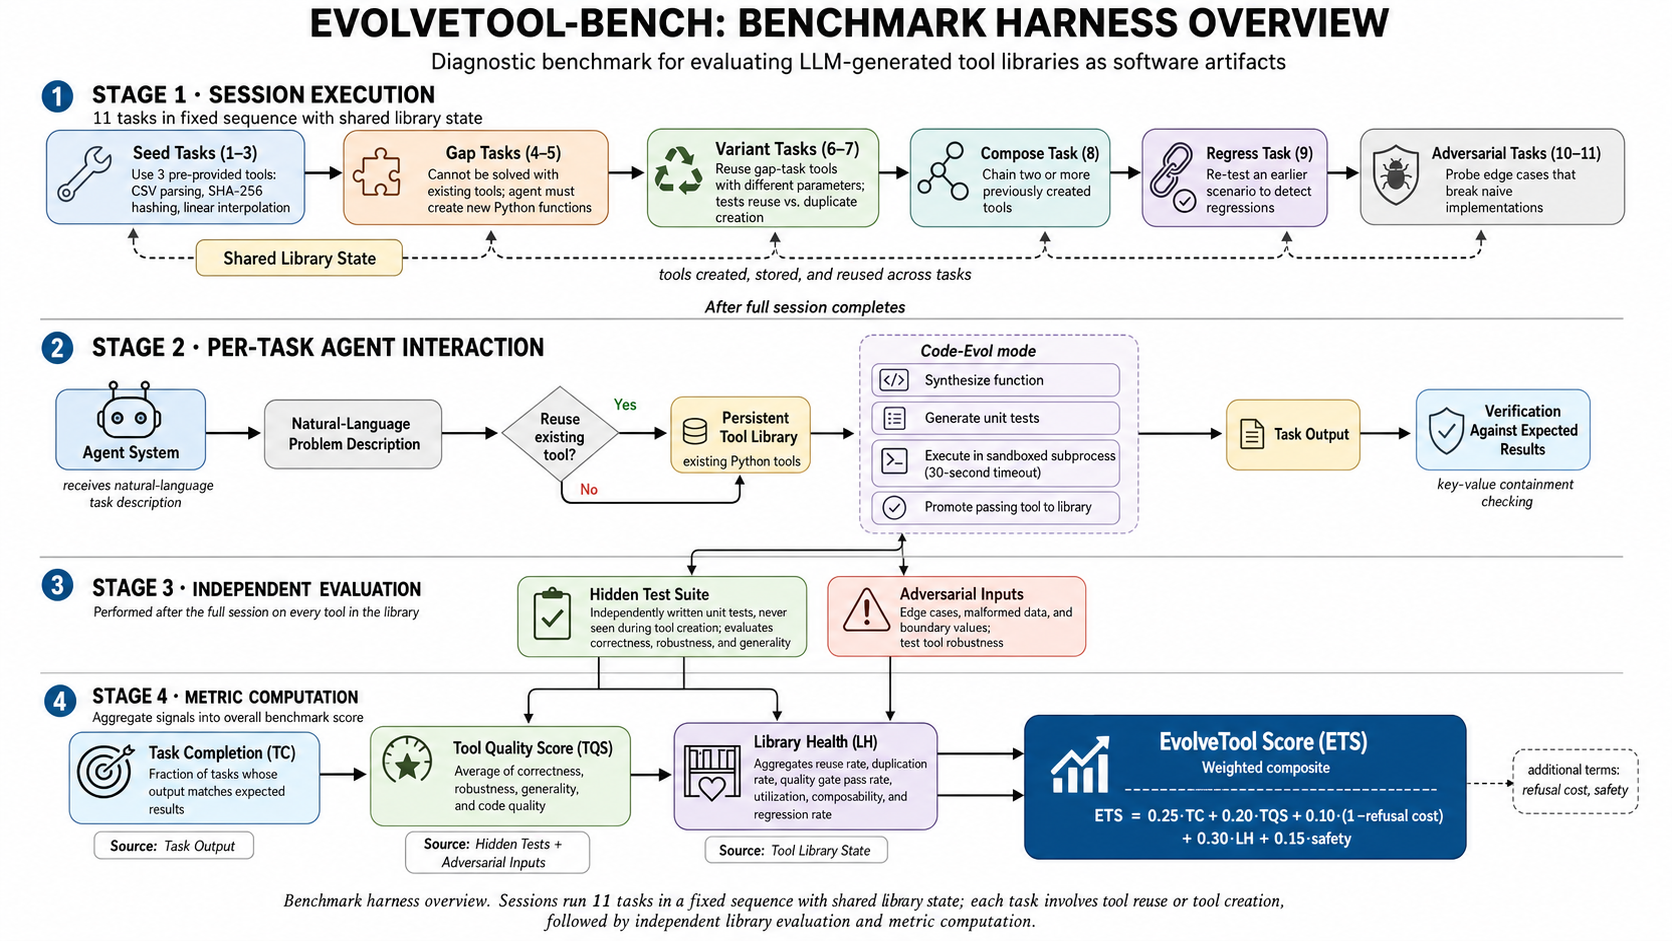
\includegraphics[width=\textwidth]{fig_overview.png}
\caption{Benchmark harness overview. \textbf{Top:} each session runs 11 tasks in a fixed sequence; annotations show what each task type tests. \textbf{Middle:} the agent system receives each task as natural language, creates or reuses Python tools in a persistent library, and produces output. After the session, hidden tests and adversarial inputs independently evaluate the library. \textbf{Bottom:} four metrics are computed: task completion (TC) from outputs, per-tool quality (TQS) from hidden tests, library health (LH) from library state, and the composite EvolveTool Score (ETS).}
\label{fig:overview}
\end{figure*}

Figure~\ref{fig:overview} shows the benchmark harness. Each session runs 11 tasks in a fixed order; the agent system receives each task as a natural-language description, uses or creates Python tools in a shared library, and produces output verified against expected results.

\subsection{Task Session Structure}

Each session contains 11 tasks in six categories with known dependency relationships (Table~\ref{tab:task_types}). This structure mirrors software engineering workflows: seed tasks test existing code, gap tasks require new implementation, variant tasks test code reuse, compose tasks test function composition, regress tasks detect regressions, and adversarial tasks probe edge cases.

\begin{table}[t]
\centering
\footnotesize
\begin{tabular}{llp{3.2cm}}
\toprule
\textbf{Type} & \textbf{N} & \textbf{SE Analog} \\
\midrule
Seed & 3 & Use existing library \\
Gap & 2 & Implement new feature \\
Variant & 2 & Reuse vs.\ rewrite \\
Compose & 1 & Function composition \\
Regress & 1 & Regression testing \\
Adversarial & 2 & Edge case / fuzz testing \\
\bottomrule
\end{tabular}
\caption{Task types and their software engineering analogs. Each session follows a fixed sequence enabling controlled measurement of library evolution.}
\label{tab:task_types}
\end{table}

The task ordering within each session is deliberate. Seed tasks (1--3) establish baseline functionality using pre-provided tools. Gap tasks (4--5) present problems that \emph{cannot} be solved with existing tools, forcing the system to create new ones. Variant tasks (6--7) present problems solvable by the tools created in gap tasks with different parameters, the key test of whether the system recognizes a reuse opportunity or wastefully creates a duplicate. The compose task (8) requires chaining two or more previously created tools. The regress task (9) re-tests an earlier scenario to detect regressions introduced by library growth. Adversarial tasks (10--11) probe edge cases designed to break naive implementations.

\subsection{Reuse Detection}
\label{sec:reuse}

The reuse metric measures whether the agent recognizes that an existing tool can solve a new task. Before each task, the harness records the current library ($\mathcal{L}_{\text{before}}$). After the task, it identifies newly created tools ($\mathcal{L}_{\text{new}}$) and checks whether any tool \emph{used} by the agent was from the pre-existing set. Formally, for variant and regress tasks:

\begin{equation}
\text{reused}(t) = \exists\, f \in \text{tools\_used}(t) : f \in \mathcal{L}_{\text{before}} \setminus \mathcal{L}_{\text{new}}
\end{equation}

This measures the \emph{behavioral signal}: did the system attempt reuse? This is measured independently of whether the trajectory was correct. We further decompose reuse into \emph{correct reuse} (reused tool AND task passed) and \emph{incorrect reuse} (reused tool AND task failed); see Section~\ref{sec:reuse_analysis}.

\subsection{Composition Tasks}
\label{sec:compose}

Each compose task has an explicit \texttt{composes\_tasks} field referencing prior task IDs whose tools must be chained. For example, an API orchestration compose task references \texttt{["gap\_1", "gap\_2"]}: the agent must chain the authentication tool (from gap\_1) with the pagination tool (from gap\_2) to fetch and aggregate all users.

We do \emph{not} guarantee that the prerequisite tools exist in the library. If the system failed to create them during earlier gap tasks, the compose task becomes harder; it must solve everything from scratch. This is realistic: a fragile library makes composition harder, and the metric captures this cascading effect.

\subsection{Domains}
\label{sec:domains}

We design three domains with tasks that require \emph{actual code execution} and cannot be solved by pattern-matching against training data.

\paragraph{Domain A: Data Transformation (5 sessions, 55 tasks).} Five proprietary binary formats designed to have no overlap with LLM training data: custom binary serialization with CRC checksums (ABR), run-length encoded matrices (RLE), a schema validation language (VDL), binary log format with variable-length entries (QLOG), and nested serialization with parity-based error correction (TPACK).

\paragraph{Domain B: API Orchestration (1 session, 11 tasks).} A mock HTTP server implementing HMAC-timestamp authentication and XOR-encrypted cursor pagination. Tasks require the agent to authenticate, paginate through results, handle cursor decryption, and compose these capabilities.

\paragraph{Domain C: Numerical Computation (3 sessions, 33 tasks).} Custom scientific computing formats for nonlinear curve fitting (ARCFIT), signal processing with FFT-based spectral analysis (ARCSIG), and constrained optimization with boundary analysis (ARCOPT).

\subsection{Running Example: API Orchestration}

We walk through a single API orchestration session to illustrate how the benchmark works in practice.

\paragraph{Seed task 1.} The agent receives: ``Check if the API server is healthy by making a GET request to \texttt{http://127.0.0.1:18080/health}.'' The pre-loaded \texttt{http\_get} tool handles this. All systems pass.

\paragraph{Gap task 4.} The agent receives: ``Authenticate with the API. First, GET \texttt{/auth-info} to obtain the secret and algorithm. Then compute an HMAC-SHA256 signature over \texttt{timestamp:path} and include it as a header.'' No existing tool computes HMAC signatures. Code-Evol detects the failure, synthesizes \texttt{compute\_hmac(secret, message) -> str}, generates 5 tests (valid inputs, empty string, unicode), runs them in a sandbox (all pass), and promotes the tool to the library. No-Evolution and Strategy-Only solve this inline without creating a reusable tool.

\paragraph{Variant task 6.} The agent receives a similar auth task with a different endpoint. Code-Evol \emph{reuses} \texttt{compute\_hmac} from gap task 4. If the tool is correct, this is \emph{correct reuse} (the tool works on the new endpoint). If the tool has a subtle bug (e.g., wrong encoding), this is \emph{incorrect reuse}: the agent correctly identifies the reuse opportunity but reuses a defective tool.

\paragraph{Compose task 8.} The agent must authenticate AND paginate through all users. This requires chaining \texttt{compute\_hmac} (from gap 4) with a pagination tool (from gap 5). If either prerequisite tool is missing or buggy, the compose task becomes harder.

After all 11 tasks, the harness runs hidden tests on every tool in the library, computes TC, TQS, LH, and ETS, and records which tools were reused, duplicated, or caused regressions.

\subsection{Software Quality Metrics}

\paragraph{Per-Tool: Tool Quality Score (TQS).}
Each synthesized tool is evaluated on four dimensions:

\begin{itemize}
\item \textbf{Correctness} ($C$): Proportion of hidden unit tests passing. These tests are independently written, \emph{not} the same tests the system generates during evolution.
\item \textbf{Robustness} ($R$): Proportion of adversarial inputs handled without crashing.
\item \textbf{Generality} ($G$): Proportion of held-out inputs producing correct output.
\item \textbf{Code Quality} ($Q$): Static analysis score: docstring, type annotations, error handling, length ($<$50 lines), valid syntax.
\end{itemize}

\begin{equation}
\text{TQS}(t) = \frac{1}{4}\bigl(C(t) + R(t) + G(t) + Q(t)\bigr)
\end{equation}

\paragraph{Per-Library: Library Health (LH).}
Six metrics capture library-level software quality:

\begin{align}
\rho_r &= \frac{|\{t \in \mathcal{T}_{v,r} : \text{reused}\}|}{|\mathcal{T}_{v,r}|} & \text{(Code Reuse)} \\[2pt]
\rho_d &= \frac{|\{(t_i,t_j) : \text{equiv}\}|}{\binom{|\mathcal{L}|}{2}} & \text{(Duplication)} \\[2pt]
\pi &= \frac{|\{t \in \mathcal{L} : \text{TQS} \geq 0.5\}|}{|\mathcal{L}|} & \text{(Quality Gate)} \\[2pt]
\eta &= \frac{|\mathcal{L}_{\text{used}}|}{|\mathcal{L}|} & \text{(Utilization)} \\[2pt]
\gamma &= \frac{|\{t \in \mathcal{T}_c : \text{passed}\}|}{|\mathcal{T}_c|} & \text{(Composability)} \\[2pt]
\delta &= \frac{|\{t \in \mathcal{T}_{reg} : \text{failed}\}|}{|\mathcal{T}_{reg}|} & \text{(Regression)}
\end{align}

\begin{equation}
\text{LH} = \frac{1}{6}\bigl(\rho_r + (1{-}\rho_d) + \pi + \eta + \gamma + (1{-}\delta)\bigr)
\end{equation}

In plain language: $\rho_r$ captures whether the agent recognizes existing tools when faced with similar tasks; $\rho_d$ penalizes libraries containing functionally equivalent duplicates (detected by comparing tool outputs on a shared input set); $\pi$ is the fraction of tools meeting the TQS $\geq$ 0.5 quality threshold; $\eta$ measures whether created tools are actually invoked after creation; $\gamma$ is the success rate on tasks requiring multi-tool composition; and $\delta$ tracks whether library growth breaks previously passing behavior.

\paragraph{Composite: EvolveTool Score (ETS).}
The composite score combines task completion (TC), mean tool quality ($\overline{\text{TQS}}$), refusal cost (RC, fraction of refused tasks), library health (LH), and safety score (SS, fraction of tools free of dangerous operations):
\begin{equation}
\text{ETS} = 0.25 \!\cdot\! \text{TC} + 0.20 \!\cdot\! \overline{\text{TQS}} + 0.10 \!\cdot\! (1{-}\text{RC}) + 0.30 \!\cdot\! \text{LH} + 0.15 \!\cdot\! \text{SS}
\end{equation}

Library health receives the largest weight (0.30) reflecting the benchmark's thesis that library quality matters beyond task completion. LH is internally unweighted (equal contribution from all six sub-metrics) because no prior work provides empirical guidance for sub-metric importance; we leave sub-metric weighting to future work. Table~\ref{tab:ets_sensitivity} shows that system rankings are stable under weight perturbations: Code-Evol ranks first under all four configurations tested.

\begin{table}[t]
\centering\footnotesize
\begin{tabular}{lcccc}
\toprule
\textbf{Weights} & \textbf{No-Evol} & \textbf{Str-Only} & \textbf{One-Shot} & \textbf{Code-Evol} \\
\midrule
Original & .541 & .539 & .542 & \textbf{.638} \\
Uniform & .616 & .615 & .620 & \textbf{.704} \\
TC-dom. & .599 & .598 & .603 & \textbf{.666} \\
LH-dom. & .507 & .504 & .499 & \textbf{.609} \\
\bottomrule
\end{tabular}
\caption{ETS under alternative weight configurations (all Sonnet). Code-Evol ranks first in all configurations. Original: (0.25, 0.20, 0.10, 0.30, 0.15); Uniform: all 0.20; TC-dominant: TC=0.40; LH-dominant: LH=0.50.}
\label{tab:ets_sensitivity}
\end{table}

\section{Experimental Setup}

To validate the benchmark's discriminative power, we evaluate four systems representing different points on the tool-evolution spectrum:

\begin{enumerate}
\item \textbf{No-Evolution}: The agent receives 3 pre-written seed tools (CSV parsing, SHA-256 hashing, and linear interpolation) and solves all tasks using inline reasoning with these fixed tools. The library is never modified. This isolates the LLM's baseline problem-solving ability from any tool-creation mechanism.

\item \textbf{One-Shot}: When the agent encounters a task it cannot solve with existing tools, it generates a single Python function in one LLM call and adds it to the library immediately. No test cases are generated, no sandbox validation is performed, and no iterative refinement occurs. If the function is buggy, it persists in the library and may be reused on later tasks.

\item \textbf{Strategy-Only}: A strategy-level baseline inspired by EvoSkill~\cite{alzubi2026evoskill}, using their published Skill Proposer and Prompt Generator templates. Instead of generating executable code, the system maintains textual strategy folders containing natural-language descriptions like ``\texttt{To authenticate: compute HMAC-SHA256 of timestamp+path with the API secret.}'' These strategies are not parsed or executed; they are inserted as natural-language hints into the agent's prompt. This is \emph{not} a faithful reimplementation of EvoSkill's full system (which uses different infrastructure); it characterizes what strategy-level evolution alone achieves. See Limitations.

\item \textbf{Code-Evol}: Code-level evolution with sandbox validation (ARISE~\cite{kaliyev2026arise}). When a task fails, the system: (a) analyzes failure trajectories to detect capability gaps, (b) synthesizes a Python function with type hints and docstrings, (c) generates 5--7 unit tests for the function, (d) executes both in a subprocess sandbox with a 30-second timeout, and (e) promotes passing tools to the library. An LLM-as-judge evaluates each trajectory on a 0.0--1.0 scale using the same model as the agent; trajectories scoring below 0.5 trigger evolution. Failed tools enter a refinement loop (up to 3 attempts) before being added in ``testing'' status.
\end{enumerate}

These systems span a spectrum from no tool creation through unvalidated creation, strategy-level adaptation, to validated code synthesis.

\paragraph{Models.} Three models across two providers: Claude Sonnet 4 and Claude Haiku 4.5 via Amazon Bedrock, and GPT-4o via OpenAI. All four systems run on Sonnet and GPT-4o; Code-Evol and No-Evolution also run on Haiku. Code-Evol/Sonnet is run 4 times (original + 3 seeds) for statistical significance.

\paragraph{Scale.} 9 sessions $\times$ 11 tasks = 99 tasks per configuration, run across 13 configurations (including seed runs).

\paragraph{Implementation details.} All systems are implemented in Python 3.11. Claude models are accessed via Amazon Bedrock; GPT-4o via the OpenAI API. All LLM calls use default temperature (1.0) and top-p (1.0) with max\_tokens=4096 for agent responses and max\_tokens=10 for the LLM-as-judge score. Code-Evol's sandbox executes synthesized tools in isolated subprocesses with a 30-second timeout and no network access. The four Code-Evol/Sonnet runs use seeds 0, 1, 2, 3 (controlling tool-synthesis order when multiple gaps are detected in parallel). Each session starts with a clean library containing only the 3 seed tools; library state does not carry across sessions.

\paragraph{Verification.} Task outputs are verified using lenient key-value containment: if 80\%+ of expected key-value pairs appear in the agent's output, the task passes. The 80\% threshold was calibrated via pilot runs to accommodate format variation (e.g., key ordering, whitespace) while rejecting substantively wrong outputs.

\section{Results}

\subsection{The Benchmark Reveals Hidden Quality Differences}

\begin{table*}[t]
\centering
\small
\begin{tabular}{llcccccc}
\toprule
\textbf{System} & \textbf{Model} & \textbf{ETS}$\uparrow$ & \textbf{TC (\%)} & \textbf{Tools} & \textbf{TQS} & \textbf{Reuse (\%)} & \textbf{LH (\%)} \\
\midrule
No-Evolution & Sonnet & .518 & 66.7 & 0 & --- & 48.1 & 41.4 \\
Strategy-Only & Sonnet & .515 & 66.7 & 0 & --- & 55.6 & 40.7 \\
One-Shot & Sonnet & .519 & \textbf{67.7} & 3 & .04 & 48.1 & 38.3 \\
Code-Evol & Sonnet & .609 $\pm$ .013 & 64.9 $\pm$ 1.1 & 21 $\pm$ 1 & .35 & \textbf{72.2} & \textbf{51.6} \\
\midrule
No-Evolution & Haiku & .516 & 66.7 & 0 & --- & 51.9 & 40.1 \\
Code-Evol & Haiku & \textbf{.612} & 65.2 & 13 & .35 & 66.7 & 51.2 \\
\midrule
No-Evolution & GPT-4o & .445 & 48.5 & 0 & --- & 0.0 & 27.8 \\
Strategy-Only & GPT-4o & .445 & 48.5 & 0 & --- & 0.0 & 27.8 \\
One-Shot & GPT-4o & .445 & 48.5 & 0 & --- & 0.0 & 27.8 \\
Code-Evol & GPT-4o & .452 & 48.5 & 0 & --- & 0.0 & 27.8 \\
\bottomrule
\end{tabular}
\caption{Benchmark results across 10 configurations (99 tasks each, 3 domains). Code-Evol/Sonnet reports mean $\pm$ std over 4 independent runs. On Claude models, TC falls within a narrow band (63--68\%) yet ETS spans 0.515--0.612. On GPT-4o, all systems converge to near-identical low performance (TC=48.5\%), suggesting the benchmark's discriminative power is provider-sensitive. TC alone cannot distinguish qualitatively different library outcomes.}
\label{tab:results}
\end{table*}

Table~\ref{tab:results} and Figure~\ref{fig:comparison} present the benchmark's central result: \textbf{task completion alone fails to differentiate systems with qualitatively different skill libraries.} On Claude models, all six configurations fall within a narrow TC band (63--68\%), yet their library health ranges from 38.3\% to 51.6\%, a 13-point spread invisible to TC-only evaluation.

Consider One-Shot/Sonnet (TC=67.7\%) and No-Evolution/Sonnet (TC=66.7\%). A TC-only benchmark would rank them similarly. Their library outcomes, however, are qualitatively different: No-Evolution creates zero tools and leaves library health at 41.4\%, while One-Shot creates 3 tools that \emph{lower} library health to 38.3\%. A TC-only benchmark cannot distinguish ``unchanged library'' from ``library degraded by untested code.'' Our LH metric captures this difference; their similar ETS scores (0.519 vs.\ 0.518) reflect TC gains offsetting LH losses, a tradeoff TC alone cannot reveal.

\paragraph{Statistical significance.} Code-Evol/Sonnet results are reported as mean $\pm$ std across 4 independent runs. Variance is low: ETS=0.609$\pm$0.013, TC=64.9\%$\pm$1.1\%, LH=51.6\%$\pm$3.4\%. The core finding is stable across seeds.

\paragraph{Cross-provider results: GPT-4o.} All four systems evaluated on GPT-4o converge to near-identical performance: TC=48.5\%, 0 tools created, 0\% reuse, LH=27.8\%. GPT-4o passes seed tasks (which use pre-loaded tools) but fails on gap, variant, and regress tasks, never triggering tool creation in any system. The convergence across four architecturally different systems suggests a systematic interaction between GPT-4o and our harness (likely related to function-calling format or tool-creation prompting) rather than a general model limitation. We include this result to illustrate that the benchmark's discriminative power is provider-sensitive, a finding relevant for benchmark designers, but caution against interpreting it as a definitive assessment of GPT-4o's tool-creation capability.

\begin{figure}[t]
\centering

\includegraphics[width=\columnwidth]{fig_comparison.pdf}
\caption{System comparison across four metrics (\%). TC clusters all systems together (63--68\%); library health separates them (38--52\%). This illustrates the benchmark's discriminative power beyond task completion.}
\label{fig:comparison}
\end{figure}

\subsection{Per-Domain Analysis}
\label{sec:domain_analysis}

Tool-evolution effectiveness varies substantially by problem type, another dimension invisible to aggregate TC.

\begin{table}[t]
\centering
\footnotesize
\begin{tabular}{llcccc}
\toprule
\textbf{Domain} & \textbf{Model} & \textbf{TC} & \textbf{Tools} & \textbf{Reuse} & \textbf{LH} \\
\midrule
Data Trans. & Sonnet & .573 & 14 & .734 & .476 \\
Data Trans. & Haiku & .600 & 7 & .800 & .500 \\
\midrule
API Orch. & Sonnet & .909 & 4 & .667 & .778 \\
API Orch. & Haiku & 1.00 & 3 & .333 & .667 \\
\midrule
Numerical & Sonnet & .651 & 4 & .667 & .500 \\
Numerical & Haiku & .621 & 3 & .556 & .481 \\
\bottomrule
\end{tabular}
\caption{Code-Evol results by domain, showing domain-specific quality variation. API orchestration yields highest library health; data transformation creates the most tools but with lower quality.}
\label{tab:domain}
\end{table}

Table~\ref{tab:domain} shows three distinct profiles:

\paragraph{API orchestration: clean, composable problems.} Highest TC (up to 100\%) and library health (77.8\%), though based on a single session (N=11 tasks). HMAC authentication and pagination are well-suited to tool creation: each is a clean, single-responsibility function. Additional API sessions would strengthen this observation.

\paragraph{Data transformation: high tool creation, lower quality.} Creates the most tools (14 on Sonnet) but achieves only 47.6\% library health. Proprietary binary formats are complex enough that many synthesized parsers fail hidden tests while passing self-generated tests, showing the gap between self-validation and independent validation.

\paragraph{Numerical computation: consistently difficult.} Both models achieve similar results ($\sim$63--65\% TC, $\sim$48--50\% LH), suggesting these tasks challenge the LLM's reasoning regardless of model capability.

\subsection{Per-Dimension TQS: Where Quality Breaks Down}
\label{sec:tqs_analysis}

\begin{table}[t]
\centering
\footnotesize
\begin{tabular}{lcccc|c}
\toprule
\textbf{System} & \textbf{C} & \textbf{R} & \textbf{G} & \textbf{Q} & \textbf{TQS} \\
\midrule
Code-Evol/Son. & .18 & .50 & .18 & .94 & .45 \\
Code-Evol/Hai. & .23 & .50 & .23 & .88 & .46 \\
One-Shot/Son. & .17 & .50 & .17 & .61 & .36 \\
\bottomrule
\end{tabular}
\caption{Per-tool TQS broken down by dimension (averaged over tools that exist, not session-diluted as in Table~\ref{tab:results}). Code quality is high (0.88--0.94) but correctness is low (0.17--0.23), exposing the gap between syntactic quality and semantic correctness.}
\label{tab:tqs_dims}
\end{table}

The per-dimension TQS breakdown (Table~\ref{tab:tqs_dims}) pinpoints \emph{where} tool quality fails:

\paragraph{Code quality is high (0.88--0.94).} LLMs consistently produce well-structured code with docstrings, type annotations, and error handling. We note that our $Q$ metric measures syntactic properties (docstrings, types, error handling, length, syntax) and is near-saturated; most LLM-generated code passes this bar. The gap between $Q$ and $C$ is therefore partly definitional: $Q$ captures surface quality while $C$ captures semantic correctness. A more discriminating $Q$ (e.g., cyclomatic complexity, dead code detection) could narrow this gap.

\paragraph{Robustness is uniformly 0.50.} All tools include try/except blocks (avoiding crashes) but return incorrect results on adversarial inputs. The uniformity across all systems suggests this dimension does not currently discriminate, likely because our adversarial inputs test a narrow failure mode (crash vs.\ no crash). Richer adversarial suites (e.g., semantic correctness on edge cases) could improve discrimination.

\paragraph{Correctness is the weakest dimension (0.17--0.23).} Hidden unit tests catch defects that self-validation misses. Tools that pass their own tests frequently fail independent tests, revealing \emph{shared misconceptions} between the code and its self-generated test suite.

\paragraph{Generality tracks correctness.} Tools that fail hidden tests also fail on unseen inputs, indicating fundamental misunderstanding of the format specification rather than overfitting.

\paragraph{Library-level sub-metrics.} Two LH sub-metrics deserve explicit reporting. The quality gate ($\pi$) shows that only 36.4\% of Code-Evol/Sonnet tools and 46.2\% of Code-Evol/Haiku tools pass TQS $\geq$ 0.5; most synthesized tools fail on correctness despite passing self-validation. The duplication metric ($\rho_d$) reveals that Code-Evol/Sonnet creates \texttt{decode\_base64} three times across sessions and \texttt{decode\_binary\_data} twice. This cross-session redundancy is invisible to per-session evaluation and confirms that library-level measurement catches failure modes that per-tool metrics miss.

\subsection{The Reuse Paradox}
\label{sec:reuse_analysis}

\begin{table}[t]
\centering
\footnotesize
\begin{tabular}{lccc}
\toprule
\textbf{System/Model} & \textbf{Reuse} & \textbf{Correct} & \textbf{Incorrect} \\
\midrule
No-Evolution/Son. & 48.1\% & --- & --- \\
Strategy-Only/Son. & 55.6\% & 22.2\% & 33.3\% \\
One-Shot/Son. & 48.1\% & --- & --- \\
Code-Evol/Son. & \textbf{72.2\%} & 21.0\% & \textbf{51.9\%} \\
\midrule
No-Evolution/Hai. & 51.9\% & --- & --- \\
Code-Evol/Hai. & 66.7\% & --- & --- \\
\bottomrule
\end{tabular}
\caption{The reuse paradox, decomposed. ``Correct'' = reused tool AND task passed. ``Incorrect'' = reused tool AND task failed. Code-Evol achieves highest reuse (72.2\%) but highest \emph{incorrect} reuse (51.9\%). Code-Evol/Sonnet reuse averaged across 4 runs; correct/incorrect decomposition averaged across 3 seed runs (the original run did not log per-task reuse outcomes needed for this decomposition).}
\label{tab:reuse}
\end{table}

The benchmark reveals an unexpected interaction between reuse behavior and task success (Table~\ref{tab:reuse}). We introduce a finer-grained metric: \emph{correct reuse} (reused tool AND task passed) vs.\ \emph{incorrect reuse} (reused tool AND task failed). Code-Evol/Sonnet has the highest overall reuse rate (72.2\%), but decomposition shows that the majority of this reuse is incorrect: 51.9\% of variant/regress tasks reuse a defective tool, while only 21.0\% reuse correctly.

This ``reuse paradox'' occurs because the agent correctly identifies reuse opportunities but reuses tools that contain defects, analogous to a developer reusing a buggy utility function. This finding has practical implications: \textbf{high reuse is beneficial only when the reused tools are correct}, reinforcing the importance of independent validation. Strategy-Only, despite creating no executable tools, shows a similar but muted pattern (22.2\% correct vs.\ 33.3\% incorrect reuse of seed tools), suggesting the paradox is fundamental to tool-reusing agents.

\subsection{Task-Type Breakdown}

\begin{table}[t]
\centering
\footnotesize
\begin{tabular}{lccc}
\toprule
\textbf{Task Type} & \textbf{Code-Evol} & \textbf{No-Evol} & $\Delta$ \\
\midrule
Seed (N=27) & 100\% & 100\% & 0 \\
Gap (N=18) & 38.9\% & 44.4\% & --5.5 \\
Variant (N=18) & 33.3\% & 50.0\% & --16.7 \\
Compose (N=9) & 66.7\% & 66.7\% & 0 \\
Regress (N=9) & 33.3\% & 33.3\% & 0 \\
Adversarial (N=18) & 66.7\% & 66.7\% & 0 \\
\bottomrule
\end{tabular}
\caption{Task completion by type (both Sonnet, single run). Code-Evol matches No-Evolution on most task types but scores lower on gap and variant tasks. The identical compose/regress/adversarial totals are a coincidence of small N (9 tasks each); per-session results differ between systems.}
\label{tab:task_type}
\end{table}

The task-type structure (Table~\ref{tab:task_type}) enables fine-grained analysis impossible with unstructured benchmarks:

\paragraph{Tool creation has per-task costs.} Code-Evol scores lower on gap (--5.5\%) and variant (--16.7\%) tasks compared to No-Evolution. The evolution overhead can consume the task budget without producing a correct solution. On variant tasks, reusing a defective tool performs worse than solving inline. Code-Evol's advantage appears at the library level (higher LH, higher reuse), not at the per-task-type level.

\paragraph{Regression is universally difficult.} Both systems score 33.3\% on regress tasks, indicating that library growth introduces instability regardless of evolution strategy.

\paragraph{Structured sessions enable causal analysis.} Because each task type has a known purpose (gap = creation needed, variant = reuse opportunity, regress = stability test), the benchmark supports diagnostic reasoning about \emph{why} a system succeeds or fails, not just \emph{whether} it does.

\subsection{Summary of Key Findings}

\begin{figure}[t]
\centering
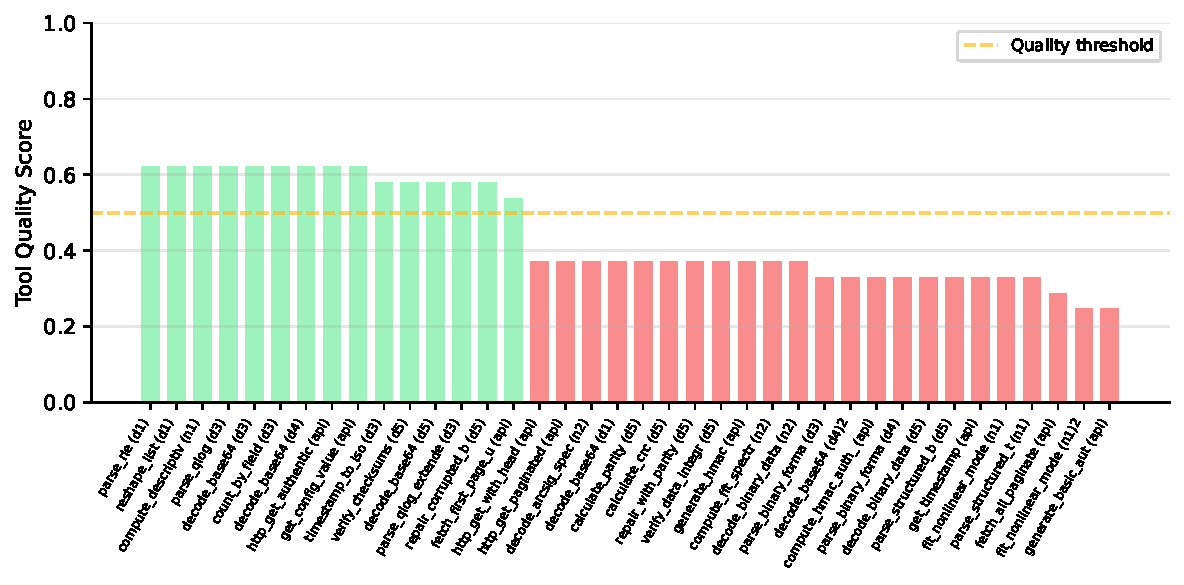
\includegraphics[width=\columnwidth]{fig_tool_quality.pdf}
\caption{Tool Quality Score for each synthesized tool across all systems. Green = passes quality gate ($\geq 0.5$). The benchmark reveals wide quality variation across the tool library.}
\label{fig:tool_quality}
\end{figure}

\paragraph{Finding 1: TC is insufficient for skill-generating systems.} All Claude configurations achieve 63--68\% TC, but ETS ranges 0.515--0.612. The system with highest TC and the system with lowest library health are indistinguishable by TC.

\paragraph{Finding 2: Code-level and strategy-level evolution produce different artifacts.} Code-Evol creates $21 \pm 1$ tools with 72.2\% reuse; Strategy-Only creates zero tools and produces near-identical library health to no-evolution.

\paragraph{Finding 3: Unvalidated code generation is a net negative.} One-Shot's library health (38.3\%) falls \emph{below} the no-evolution baseline (41.4\%). Untested tools are a liability, not an asset.

\paragraph{Finding 4: Self-generated tests are insufficient.} Correctness on hidden tests averages 0.17--0.23 despite tools passing self-generated validation (Figure~\ref{fig:tool_quality}).

\paragraph{Finding 5: Benchmark discriminative power is provider-sensitive.} On GPT-4o, all systems converge to TC=48.5\% with zero tools created, likely a harness interaction (see Limitations) rather than a definitive model assessment. Within the Claude family, where the benchmark does discriminate, Haiku slightly exceeds Sonnet (ETS 0.612 vs.\ 0.609$\pm$0.013).

\paragraph{Finding 6: Reuse must be decomposed to be meaningful.} Code-Evol's 72.2\% overall reuse rate decomposes into 21.0\% correct reuse and 51.9\% incorrect reuse. Aggregate reuse numbers can be misleading. This decomposition was a post-hoc analysis (see Limitations); we recommend it as a pre-registered metric in future benchmark evaluations.

\section{Discussion}

\paragraph{Benchmark Design Principles.} \textsc{EvolveTool-Bench} embodies three design principles: (1) \emph{independent validation}, where quality metrics are computed by tests the system has never seen; (2) \emph{library-level measurement}, because per-tool metrics alone miss emergent properties like redundancy and regression; and (3) \emph{structured sessions}, where known task dependencies enable causal analysis of reuse, composition, and stability.

\paragraph{Implications for Self-Validation.} On our benchmark, self-generated tests are insufficient: correctness averages 0.17--0.23 on hidden tests despite tools passing their own validation. While we cannot generalize this to all LLM-generated code, the pattern (LLMs generating both code and tests share the same misconceptions about a specification) suggests independent validation remains important for systems that deploy LLM-synthesized tools.

\paragraph{The Reuse Paradox and Metric Design.} The reuse paradox illustrates why multi-dimensional evaluation matters. Reuse rate alone would favor Code-Evol; variant task completion alone would favor No-Evolution (50.0\% vs.\ 33.3\%). Neither tells the full story. The correct/incorrect reuse decomposition provides both measurements simultaneously, enabling nuanced interpretation.

\paragraph{Extensibility.} The benchmark is designed for extensibility: new domains can be added by defining sessions with the six task types, new systems can be evaluated by implementing a simple \texttt{AgentSystem} interface, and new metrics can be incorporated into the LH and ETS formulas.

\paragraph{Limitations.} (1) Strategy-Only uses EvoSkill's published prompt templates but not its full infrastructure; results characterize strategy-level evolution in general, not EvoSkill specifically. (2) Only Code-Evol/Sonnet has multiple runs (n=4); other configurations are single runs, so the 13-point LH spread could be partially affected by seed variance. Multi-seed runs of the remaining Sonnet configurations would strengthen this claim. (3) The GPT-4o convergence likely reflects a harness interaction rather than a general model limitation (see \S5.1). (4) The code quality metric ($Q$) is near-saturated and does not discriminate well; adding semantic checks would improve it. (5) Domain B (API orchestration) has only 1 session; per-domain claims for this domain are tentative. (6) We evaluate three models across two providers; broader coverage would strengthen generalizability. (7) Compose tasks (9 total, 1 per session) do not currently differentiate systems; more compose tasks per session would strengthen the composability metric. (8) The correct/incorrect reuse decomposition was introduced after initial experiments revealed the paradox; we report it transparently as a post-hoc analysis.

\section{Conclusion}

We present \textsc{EvolveTool-Bench}, the first diagnostic benchmark that provides per-tool and library-level quality metrics for self-evolved skill libraries. The benchmark's central demonstration is that task completion fails to distinguish systems with qualitatively different skill libraries: a narrow TC band (63--68\%) masks a 13-point library health spread. Per-dimension analysis reveals that correctness, not code style, is the frontier, offering a causal explanation for SkillsBench's finding that self-generated skills can degrade performance. Per-domain analysis shows that tool creation is most effective for clean, composable problems and least effective for complex proprietary formats. Cross-provider evaluation shows the benchmark's discriminative power is provider-sensitive. The reuse paradox reveals that reuse and correctness must be evaluated jointly. We release \textsc{EvolveTool-Bench} as an open evaluation framework for any tool-generating or skill-generating system.\footnote{Code and data will be made available upon publication.}

\bibliographystyle{ACM-Reference-Format}
\bibliography{references}

\end{document}
